\chapter{UML-diagrams}
\label{UML}

% Cannot get this picture to be pretty
\section{MVC}
\label{UML-MVC}
\begin{figure}[h!]
\centering
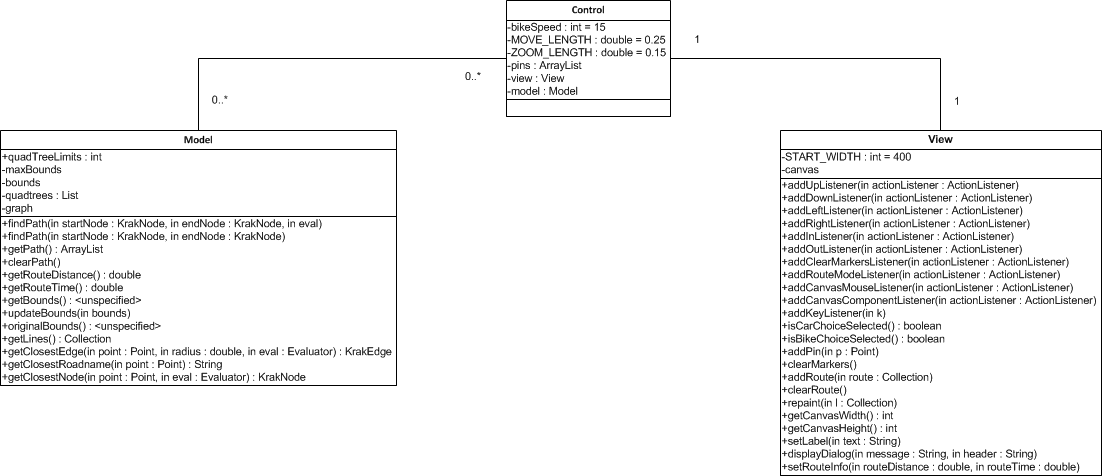
\includegraphics[width=1.25\linewidth]{images/mvc-map}
\caption{UML of the MVC architecture in our Map program}
\label{mvc-map}
\end{figure}

Figure \ref{mvc-map} shows our implementation of the MVC architecture. Because we 
have exactly one window, we chose to name our view and controller ``\class{View}'' and 
``\class{Control}'', respectively. The same goes for the models. We only have one data 
source (Krak's data-set), and because of that our model is called ``\class{Model}''. We could 
have named these three classes something different that may have been more meaningful 
in terms of the \class{Map of Denmark} context, but we chose these name in order to make 
our architecture clear.

% This section (until next section) is quite ``loose'' / quite bad.
We wanted to keep the models as ``skinny'' as possible, 
although our \class{Model} is quite long. But the amount of (public) methods is small, so 
looking at it from outside, it is a skinny model. The reason we wanted to keep the models 
skinny, is because it isn't the model's responsibility to deliver the same data in different ways, 
do a lot of calculations or stuff like that. It only acts like a ``middle-man'', delivering data to 
other classes. If some class want the data in another way, they will need to convert it 
themselves.

Data processing takes place in \class{Control}. It translates data that the model can 
understand, to something the view can understand, and the other way around. For 
an example the view only knows about pixels, but it has no idea about UTM 
coordinates. The model only knows about UTM coordinates, but doesn't know anything 
about pixels. So for getting these two to communicate, we need to convert pixels to 
UTM and vice versa.

We created some helper-classes (\class{PointMethods} and \class{RectangleMethods}), 
which are located in the \class{utils} package. These take care of checking whether a point 
is within the maximal bounds of the map, converting a pixel coordinate to a UTM coordinate 
and vice versa. We did this for being able to do this in several files, without the need to have 
duplicate code. For our program right now, this isn't really a problem, as we only have one 
model, one controller and a view. But if we were to have more, we would either need to copy 
these helper-methods into the other classes (BAD), or put them in a separate class. But even 
though we only have one of each, the helper-classes are still an advantage, as they make the 
code cleaner and easier to maintain and test, as we can test these helper-classes.

So in essence, we have two parts (the model and the view) that need to communicate 
somehow, in order to display the data on the screen. But they speak different languages, so 
we put in a middle-man (the controller), responsible for the communication between the two.

\section{Control flow}
\label{UML-CF}
The easiest way to understand MVC and how the individual parts talk together, is by using 
an example. Let us say the user has already clicked the map and placed a pin. Now the 
user clicks on the map again to place another pin.

% Same as the other picture
\begin{figure}[h!]
\centering
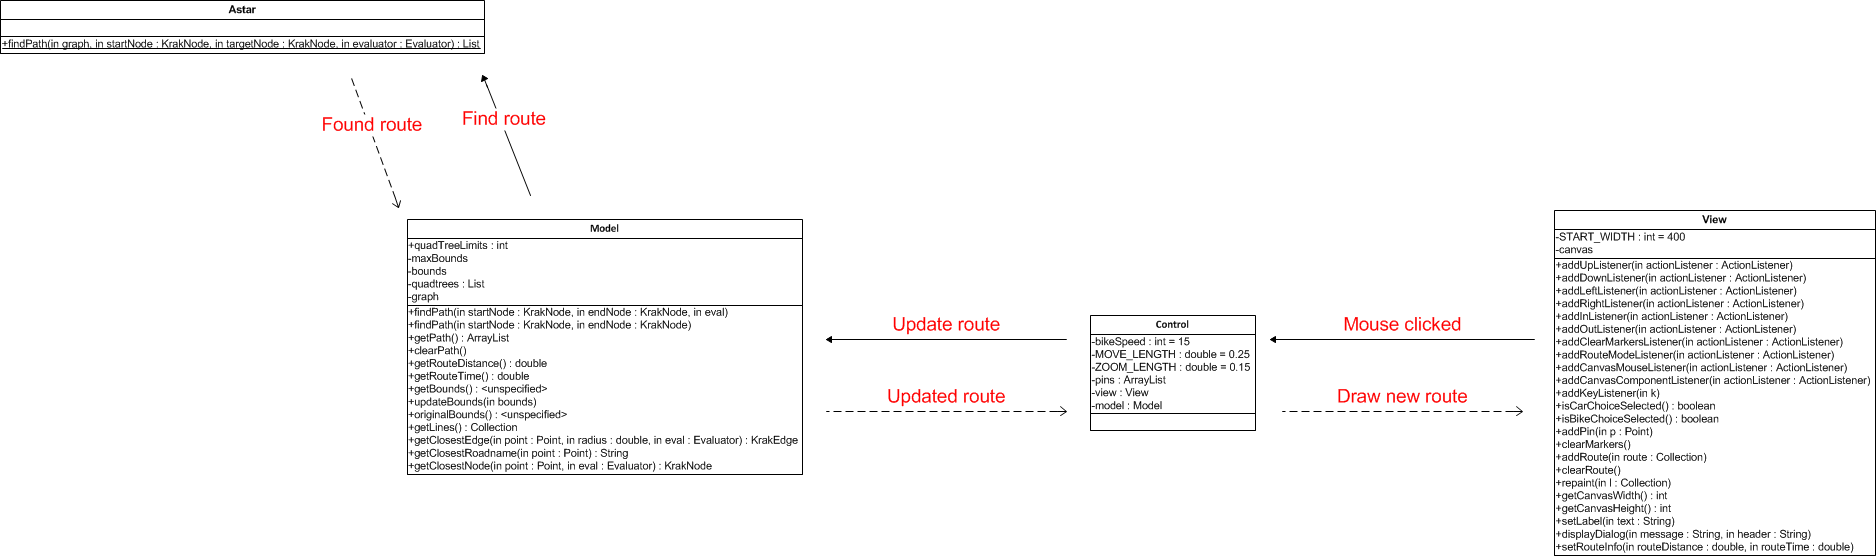
\includegraphics[width=1.25\linewidth]{images/control-flow}
\caption{The basic control flow of our Map program}
\label{control-flow}
\end{figure}
 
 % Longer
The controller has placed listeners in the view, so when a MouseClicked event is thrown, 
the controller is called. First it checks if there is another pin at the spot of the click. If there 
is, this will be removed, and the model is told to clear the route. If there is still over two 
pins placed, the model is asked to calculate a new route.

If there isn't a pin where the user clicks, we place a new pin. If the user has placed two or 
more pins, the controller calls its own findPath-method from point 1 to point 2, point 2 to 
point 3 and so on. The findPath()-method tells the model to find a path between the two 
points given.

The model then asks a helper-class to find a path, using the A* algorithm, and provides it 
with the graph and the two points. When a path is found, it is saved in the model, ready 
for use in the controller.

The final step is getting the view to draw the route. The controller gets ready for a repaint, 
by fetching the route from the model. Then it passes this route to the view's repaint-method, 
and the view paints the road.